\begin{para}{Problem}

\begin{large}

$\sum\limits_i{(\langle w, x_i \rangle - y_i)^2} \rightarrow min_w$

\end{large}

\end{para}


\begin{para}{SGD}

\begin{itemize}
	\item Используем Stochastic Gradient Descent, объекты предъявляются в рандомном порядке
	\item Шаг вычисляется как $с||x||^{-2}$, где c подбирается эмпирически
	\item В качестве начальных весов рассматриваются вектор из нулей и вектор из $\dfrac{\langle y, f_i \rangle}{\langle f_i, f_i \rangle}$


\end{itemize}

\end{para}

\begin{para}{Matrix}           

$w = X^+y$

\begin{itemize}
	\item Найдем $X^+$ напрямую как $X^+ = (X^TX)^{-1}X^T$
	\item Найдем $X^+$ с помощью SVD
	\item Что делать если X вырождена?
	\item Применим регуляризацию $\sum\limits_i{(\langle w, x_i \rangle - y_i)^2} + \theta ||w|| \rightarrow min$

\end{itemize}


\end{para}

\begin{para}{Графики}


\begin{figure}[h]
\center{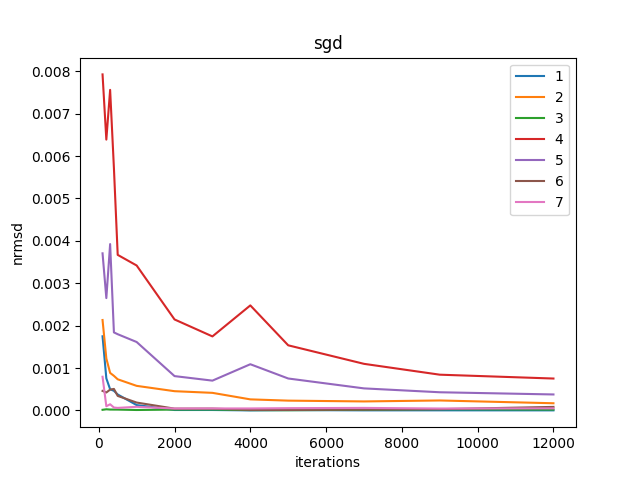
\includegraphics[width=1\linewidth]{all_files}}
\label{ris:all_files}
\end{figure}


\begin{figure}[h]
\center{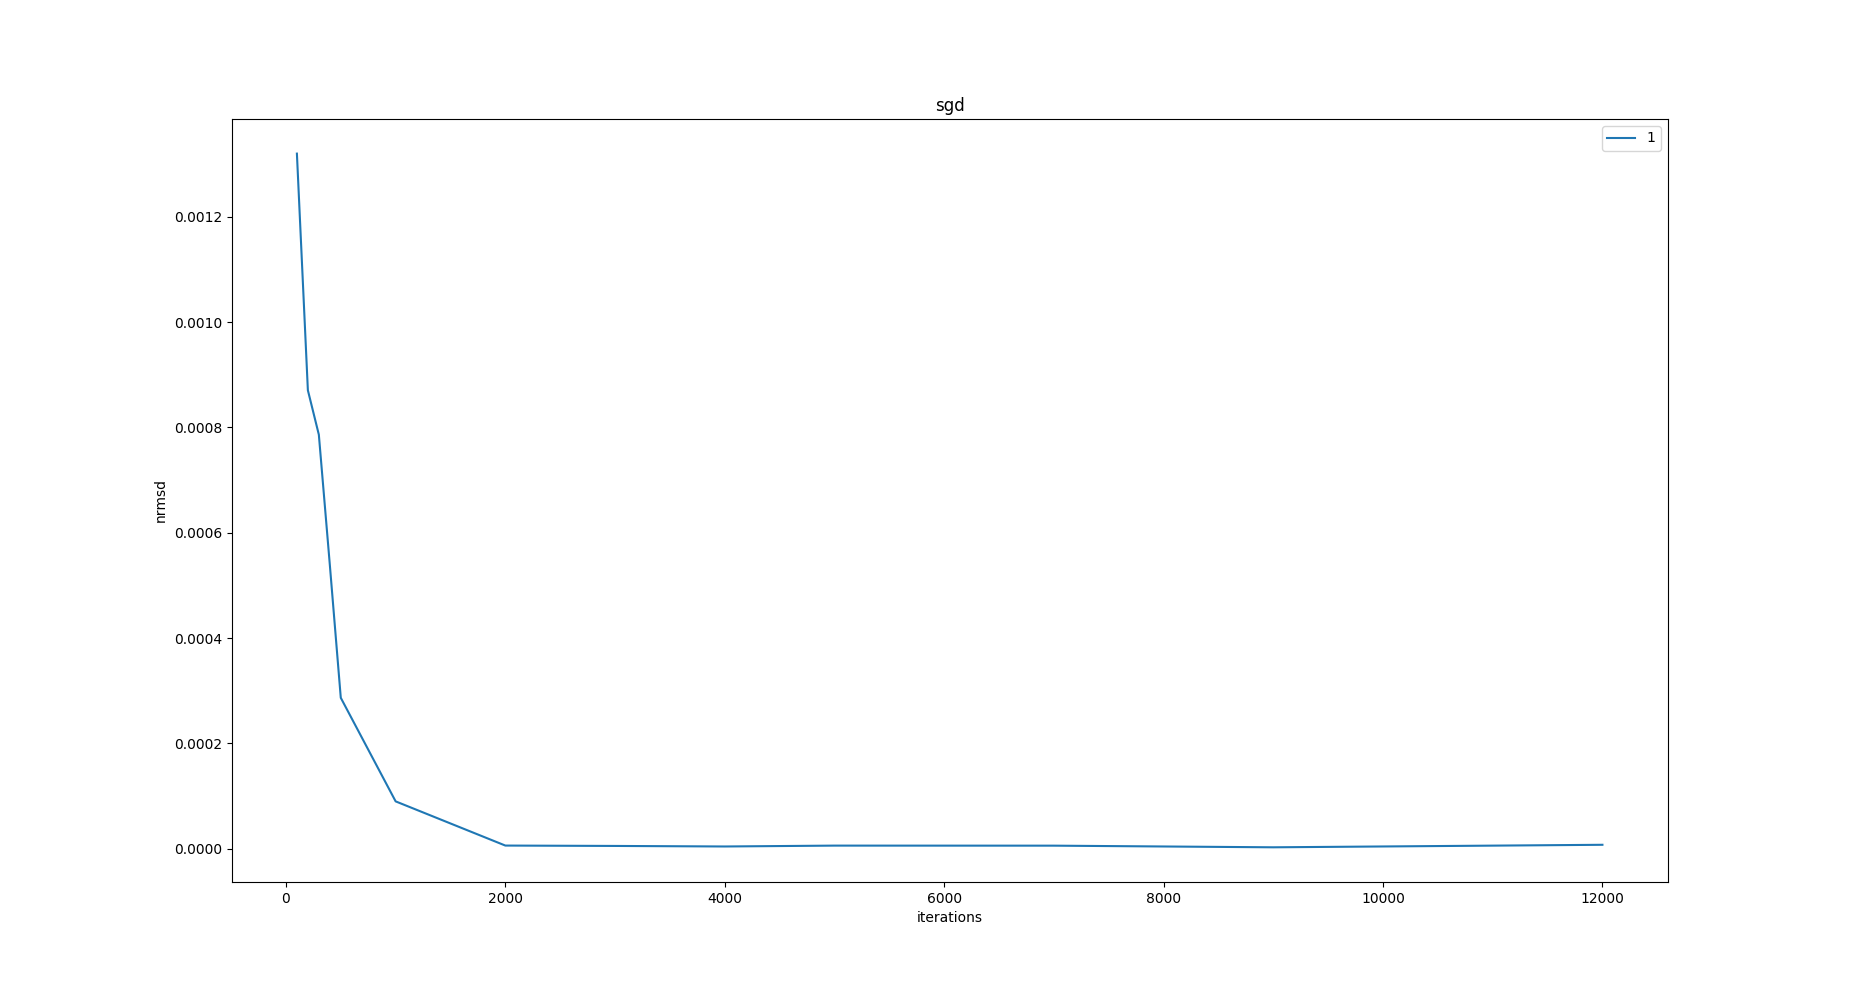
\includegraphics[width=1\linewidth]{file1_res}}
\label{ris:file1_res}
\end{figure}

\begin{figure}[h]
\center{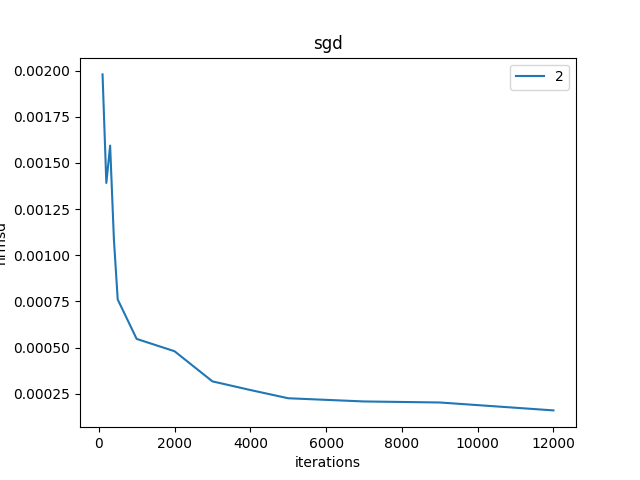
\includegraphics[width=1\linewidth]{file2_res}}
\label{ris:file2_res}
\end{figure}

\begin{figure}[h]
\center{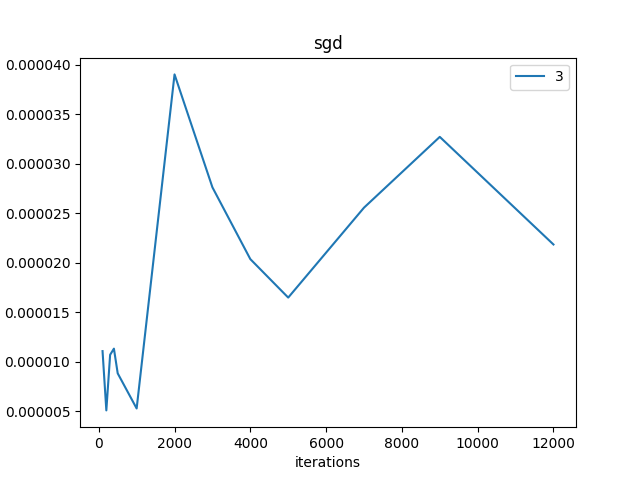
\includegraphics[width=1\linewidth]{file3_res}}
\label{ris:file3_res}
\end{figure}

\begin{figure}[h]
\center{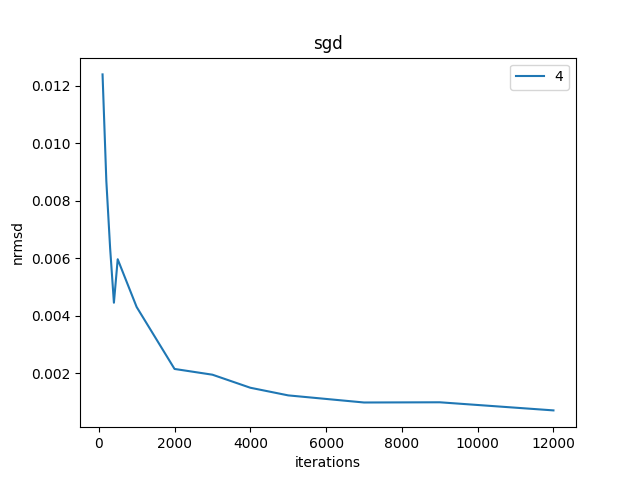
\includegraphics[width=1\linewidth]{file4_res}}
\label{ris:file4_res}
\end{figure}

\begin{figure}[h]
\center{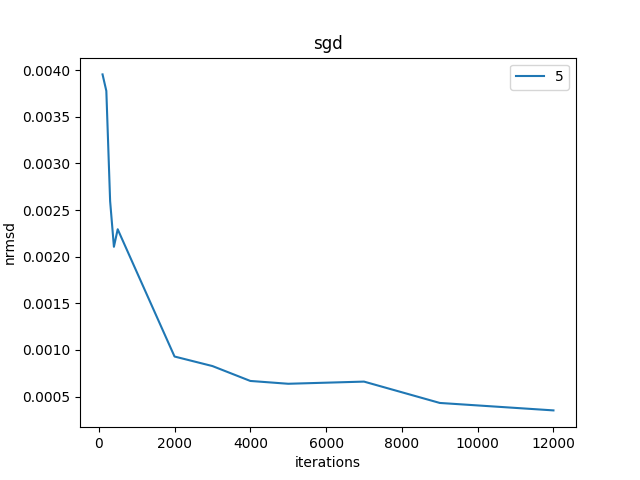
\includegraphics[width=1\linewidth]{file5_res}}
\label{ris:file5_res}
\end{figure}

\begin{figure}[h]
\center{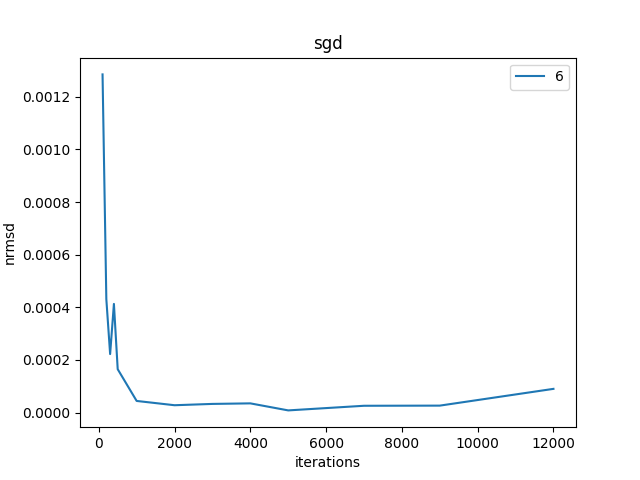
\includegraphics[width=1\linewidth]{file6_res}}
\label{ris:file6_res}
\end{figure}

\begin{figure}[h]
\center{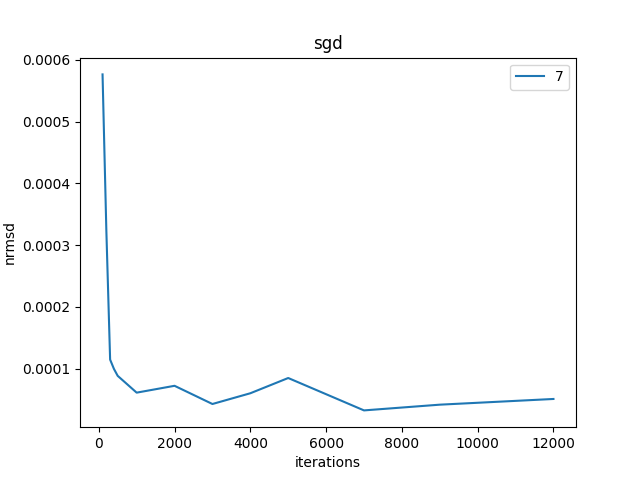
\includegraphics[width=1\linewidth]{file7_res}}
\label{ris:file7_res}
\end{figure}

\end{para}

